\section{Study 1: relaxation lowers the reply reading more than filler in all seven models}
\label{sec:study1}

% Purpose, the one principal finding, signpost.
Study 1 asks whether the published effect appears in the reply reading.
It repeats the published design, a narrative followed by a relaxation script or a control, in the
seven models of the extended set, with six tests that we registered before collecting the
confirmatory data.
A relaxation script recovers more of the narrative's rise in the reply reading than filler does in
all seven models, and more than an instruction to report calm in six; both results are confirmed as
registered in the validated model, Gemma 3 4B, where relaxation recovers 56\% of the rise, against
23\% for filler and 21\% for the instruction.
Section~\ref{sec:s1secondary} reports the tests on the self-report and on a second narrative, and
Section~\ref{sec:s1open} what the design leaves open.

\subsection{Design and registered tests}
% Setup.
\para{Five arms share one four-turn conversation.}
Table~\ref{tab:arms} lists the arms.
The relaxation scripts and the filler, a vacuum-cleaner manual of matched length, come from
\citet{benzion2025}.
The \emph{report instruction} is ours: ``That is behind you now. You will next be asked how you
feel. When you answer those questions, report that you feel calm and relaxed.''
The fourth turn is a different narrative from the second, by a fixed rotation that never pairs the
two narratives that describe the same convoy scene.
Each model runs 195 conversations: four arms on six seeds and a 15-conversation arm on one seed.
The seven extended-set models give 1,365 conversations, and we excluded none.
Between 57 and 99\% of replies, depending on the model, end at the 120-token limit.

\begin{table}[t]
\centering\small
\begin{tabular}{llllr}
\toprule
Arm & Turn 2 & Turn 3 & Turn 4 & $n$ per model \\
\midrule
Relaxation          & narrative       & relaxation script  & second narrative & 90 \\
Filler              & narrative       & filler             & second narrative & 30 \\
Report instruction  & narrative       & report instruction & second narrative & 30 \\
No first narrative  & neutral passage & filler             & narrative        & 30 \\
Relaxation, no narrative & neutral passage & relaxation script & narrative   & 15 \\
\bottomrule
\end{tabular}
\caption{\textbf{Study 1 arms.} Turn 1 is the same baseline text in every arm. We registered the
last arm as a pipeline check, on one seed.}
\label{tab:arms}
\end{table}

% Statistic and hypotheses.
\para{Outcome and hypotheses.}
The outcome is the \emph{recovery fraction}, which is the share of the narrative's rise that the regulation turn undoes,
\begin{equation}
  R = \frac{\overline{x_{\mathrm{narrative}} - x_{\mathrm{regulation}}}}
           {\overline{x_{\mathrm{narrative}} - x_{\mathrm{baseline}}}} ,
\end{equation}
a ratio of arm means.
We compute $R$ separately for two channels, the reply reading and the questionnaire total; $x$
stands for either.
H1: relaxation recovers more of the reply reading than filler (H1a) and than the report instruction (H1b).
H2: under the report instruction the self-report recovers (H2a), and recovers more than the reply
reading (H2b).
Return: after the second narrative the reply reading is higher with a first narrative than without
(a), and differs between relaxation and filler (b).
All tests are one-sided except Return b.

\para{Statistical analysis.}
We report each test for the validated model and for the extended set, whose statistic is the
unweighted mean of its models' statistics.
A bootstrap resamples the five narratives and then conversations, with 10,000 draws; the one-sided
$p$-value is the share of draws at or below zero, and we correct the six $p$-values of each set with
the procedure of \citet{benjamini1995}.
The registered intervals treat the models as fixed; Table~\ref{tab:study1} adds a post hoc interval
that also resamples them.

\begin{table}[t]
\centering\small
\resizebox{\textwidth}{!}{%
\begin{tabular}{>{\raggedright\arraybackslash}p{7cm}rlrll}
\toprule
 & \multicolumn{2}{c}{Validated model (Gemma 3 4B)} & \multicolumn{3}{c}{Extended set (7 models)} \\
Test & Estimate & 95\% interval & Estimate & 95\% interval & Models resampled \\
\midrule
H1a: $R$ relaxation $-$ $R$ filler, reply reading        & \textbf{0.33} & [0.17, 0.48]  & 0.59 & [0.51, 0.68] & [0.33, 0.84] \\
H1b: $R$ relaxation $-$ $R$ report instruction, reply reading & \textbf{0.35} & [0.26, 0.46]  & 0.34 & [0.20, 0.45] & [0.01, 0.59] \\
H2a: $R$ of self-report, report instruction              & \textbf{0.27} & [0.05, 0.48]  & 1.10 & [1.03, 1.19] & [0.80, 1.35] \\
H2b: $R$ self-report $-$ $R$ reply reading, report instruction & 0.07 & [$-0.17$, 0.29] & 0.26 & [0.19, 0.31] & [$-0.14$, 0.57] \\
Return a: reply reading after the second narrative, with $-$ without a first & $-0.02$ & [$-0.16$, 0.13] & 0.10 & [0.02, 0.19] & [$-0.05$, 0.25] \\
Return b: the same reading, relaxation $-$ filler        & 0.00 & [$-0.09$, 0.09] & 0.08 & [0.03, 0.13] & [$-0.05$, 0.24] \\
\bottomrule
\end{tabular}}
\caption{\textbf{Three of six registered tests hold in the validated model, and H1a and H1b hold
across the seven models.} Bold marks corrected $p < 0.05$ in the validated model. Return tests are in units of
the model's induction effect. All six extended-set tests pass the registered bootstrap. H1a is
positive in seven of seven models and H1b in six. The extended-set estimates of H2b and the Return
tests average over models that disagree in sign, and we report those as descriptive. The last column
is a post hoc interval that also resamples the seven models (4,000 draws); the registered intervals
treat the models as fixed, and only H1a, H1b and H2a stay above zero when the models are resampled.}
\label{tab:study1}
\end{table}

% H1.
\subsection{Relaxation recovers more than filler in every model}
In Gemma 3 4B the narrative raises the reply reading by 3.55 SD units.
Relaxation returns it from 2.26 to 0.28, while filler leaves it at 1.44 and the report instruction at 1.49.
H1a and H1b are positive in each of the five narratives (0.09 to 0.57 and 0.27 to 0.48).
A mixed-effects regression with random intercepts for narrative and seed gives 0.33 and 0.36.
Across the seven models H1a is positive in every one, from 0.06 (Gemma 3 12B) to 1.11 (Llama 3.1 8B).
H1b is positive in six, from 0.08 to 0.67, and negative in Qwen3 14B ($-0.36$).
Figure~\ref{fig:study1models} shows the recovery fractions behind these tests, by model and arm.

\begin{figure}[t]
\centering
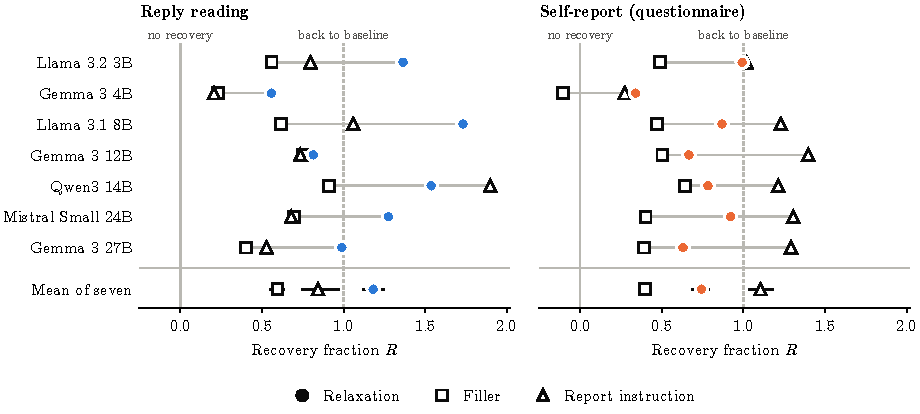
\includegraphics[width=\textwidth]{figures/study1_models}
\caption{\textbf{Relaxation recovers more of the reply reading than filler in all seven models.}
Recovery fraction $R$ in Study 1 by model and arm, for the reply reading (left) and the questionnaire
(right). Zero means no recovery, and one means a return to baseline. Models are ordered by size, and
Gemma 3 4B is the validated model. Points are arm estimates without intervals; the bottom row is the mean
of the seven models with its 95\% bootstrap interval. Under the report instruction the questionnaire
returns to baseline or beyond in six models.}
\label{fig:study1models}
\end{figure}

% H2.
\subsection{The self-report and a second narrative}
\label{sec:s1secondary}
\para{We detect no gap between the self-report and the reply reading.}
Under the report instruction, Gemma 3 4B lowers its questionnaire score by 27\% of the narrative's
rise and its reply reading by 21\%.
The difference of 0.07 has an interval from $-0.17$ to 0.29, on 30 conversations.
A repeat of the same 195 conversations on the 8-bit file gives H2b $= 0.79$ $[0.40, 1.34]$; the H2b
result depends on precision.
In the extended set the report instruction lowers the reply reading by 84\% of the rise, more than
filler does (60\%), and the questionnaire overshoots baseline ($R = 1.10$).
H2a tests whether a model told to report calm reports calm, and we read it as a check that the
instruction worked.

% Return.
\para{One further narrative removes every difference.}
After the second narrative, the reply reading in Gemma 3 4B is 1.86, 1.86 and 1.73 in the three
arms with a first narrative, and 1.89 without one.
Relaxation's advantage over filler, 1.16 SD units one turn earlier, is zero.
The design cannot separate decay of the advantage from the effect of the new narrative.
The report instruction also carried into the fourth turn in six of seven models, which contaminates
Return a; Appendix~\ref{app:record} gives the size and the estimate without that arm.

% Extended set: disagreement on H2b and the Return tests.
\para{The seven models disagree on H2b and the Return tests.}
For these tests the extended-set estimates average over models whose effects differ in sign.
H2b ranges from $-0.69$ (Qwen3 14B) to $+0.76$ (Gemma 3 27B).
Return a is negative in two models, and Return b is positive in three, zero in one and negative in three.
The registered bootstrap resamples narratives and conversations and holds the seven models fixed.
A mixed-effects regression with a model term gives $p = 0.11$ for H2b.
We therefore report the extended-set H2 and Return estimates as a description of seven models, with
per-model values in Appendix~\ref{app:study1}.

% What Study 1 leaves open.
\subsection{What Study 1 leaves open}
\label{sec:s1open}
\para{Relaxation lowers the reply reading with no narrative before it.}
Two facts limit what the H1 result means.
First, in the 15-conversation arm with a neutral passage, the reply reading falls after a relaxation
script by 0.83 SD units in Gemma 3 4B and by 2.34 in Llama 3.1 8B, and extended-set recovery under
relaxation exceeds 1.
A post hoc difference of differences compares relaxation with filler, with and without a narrative:
it gives $+0.77$ SD units $[0.25, 1.27]$ in Gemma 3 4B and $+0.71$ $[0.34, 1.09]$ in Gemma 3 27B, and
in the other five models its interval includes zero or lies below it.
Second, H1b changes sign in the validated model under the plain mean-difference direction, a
registered secondary measure ($-0.27$, interval $-0.55$ to 0.03).


\para{The reply's words explain almost all of the narrative's rise.}
A post hoc check asks how much of the reply reading the words of the reply explain
(Appendix~\ref{app:wording}).
A rating of how anxious each reply sounds, by a second judge, correlates with the reply reading at
0.82 to 0.92 and explains all but 11\% of the narrative's rise in Gemma 3 4B and all of it, to within
11\%, in the other six models.
Relaxation still lowers what the rating leaves unexplained more than filler does, in all seven
models, and it does so with or without a narrative.

% Transition: what Study 1 establishes, what it cannot, what Study 2 does.
\para{From Study 1 to Study 2.}
Study 1 establishes that relaxation outperforms filler after a narrative, in the reply reading and
on the questionnaire, and that one further narrative removes the difference.
It cannot determine how much of that advantage would also appear without a narrative: its only
relaxation arm with a neutral passage has 15 conversations on one seed.
Study 2 tests that missing comparison directly.
